%==============================================================================
%  Find in Images — Project Report
%
%  Modular LaTeX project. This file holds the preamble + document scaffolding;
%  each section lives in its own file under sections/ and is pulled in with
%  \input below. Build with:  ./build.sh   (or: tectonic -X compile main.tex)
%==============================================================================
\documentclass[11pt,a4paper]{article}

% --- Engine-aware font setup (works under both XeTeX/Tectonic and pdfLaTeX) ---
\usepackage{iftex}
\ifPDFTeX
  \usepackage[T1]{fontenc}
  \usepackage[utf8]{inputenc}
  \usepackage{lmodern}
\else
  \usepackage{fontspec}
\fi

% --- Layout & typography ------------------------------------------------------
\usepackage[margin=1in]{geometry}
\usepackage{microtype}
\usepackage{parskip}            % block paragraphs, modern look
\usepackage{setspace}
% \onehalfspacing   % dropped — single spacing keeps the report compact
\setlength{\emergencystretch}{3em}   % soak up minor overfull lines (inline \code, URLs)

% --- Color & graphics ---------------------------------------------------------
\usepackage{graphicx}
\usepackage{xcolor}
\definecolor{accent}{HTML}{1F6FB2}     % links / headings accent
\definecolor{codebg}{HTML}{F6F8FA}
\definecolor{codekw}{HTML}{8250DF}
\definecolor{codestr}{HTML}{0A7D33}
\definecolor{codecmt}{HTML}{6A737D}
\definecolor{rulegray}{HTML}{D0D7DE}

% --- Tables & lists -----------------------------------------------------------
\usepackage{booktabs}
\usepackage{array}
\usepackage{tabularx}
\usepackage{enumitem}
\setlist{itemsep=2pt,topsep=4pt}

% --- Section heading styling --------------------------------------------------
\usepackage{titlesec}
\titleformat{\section}{\Large\bfseries\color{accent}}{\thesection}{0.7em}{}
\titleformat{\subsection}{\large\bfseries}{\thesubsection}{0.6em}{}

% --- Headers / footers --------------------------------------------------------
\usepackage{fancyhdr}
\pagestyle{fancy}
\fancyhf{}
\renewcommand{\headrulewidth}{0.4pt}
\fancyhead[L]{\small\itshape Find in Images}
\fancyhead[R]{\small\itshape Project Report}
\fancyfoot[C]{\thepage}

% --- Math & diagrams ----------------------------------------------------------
\usepackage{amsmath}
\usepackage{tikz}
\usetikzlibrary{shapes.geometric, arrows.meta, positioning, fit, backgrounds}

% --- Code listings ------------------------------------------------------------
\usepackage{listings}
\lstdefinestyle{js}{
  basicstyle=\ttfamily\small,
  backgroundcolor=\color{codebg},
  keywordstyle=\color{codekw}\bfseries,
  stringstyle=\color{codestr},
  commentstyle=\color{codecmt}\itshape,
  numbers=left, numberstyle=\tiny\color{codecmt}, numbersep=8pt,
  frame=single, framerule=0.4pt, rulecolor=\color{rulegray},
  breaklines=true, breakatwhitespace=true,
  showstringspaces=false, tabsize=2,
  language=Java,                                  % close enough for JS keywords
  morekeywords={const,let,async,await,function,of,new,class,export,import,from},
  captionpos=b, xleftmargin=14pt, framexleftmargin=14pt,
}
\lstset{style=js}

% --- Captions -----------------------------------------------------------------
\usepackage{caption}
\captionsetup{font=small,labelfont=bf,labelsep=period}

% --- Bibliography (classic BibTeX; Tectonic runs bibtex internally, no biber) -
\usepackage{cite}

% --- Hyperlinks (load late) ---------------------------------------------------
\usepackage[hidelinks]{hyperref}
\hypersetup{
  colorlinks=true,
  linkcolor=accent, citecolor=accent, urlcolor=accent,
  pdftitle={Find in Images — Making Scanned PDFs Searchable in Chrome's Own Viewer with On-Device OCR},
  pdfauthor={Suhani Pandey},
}

% --- Handy macros -------------------------------------------------------------
\newcommand{\code}[1]{\texttt{#1}}
\newcommand{\proj}{\textsc{Find in Images}}

%==============================================================================
\begin{document}

% ---------- Title page --------------------------------------------------------
\begin{titlepage}
  \centering
  \vspace*{1.5cm}

  {\Large\bfseries\color{accent} Searchable Documents Project\par}
  \vspace{0.4cm}
  {\color{rulegray}\rule{0.6\textwidth}{1pt}}\par
  \vspace{1.2cm}

  {\Huge\bfseries Find in Images\par}
  \vspace{0.8cm}
  {\LARGE Making Scanned PDFs Searchable\\[0.3em]
   in Chrome's Own Viewer with On-Device OCR\par}

  \vspace{2.2cm}
  {\large\bfseries Suhani Pandey\par}
  \vspace{0.3cm}
  {\normalsize A Chrome Extension (Manifest V3)\par}

  \vfill


  \vspace{1.2cm}
  {\large \today\par}
\end{titlepage}

\tableofcontents
\thispagestyle{fancy}
\clearpage

% ---------- Body --------------------------------------------------------------
% ---------- Front matter ------------------------------------------------------
\begin{abstract}
\noindent
Scanned PDFs and image-based documents are ubiquitous, yet many of them carry no
machine-readable text, so the browser's familiar ``find on page''
($\mathrm{Ctrl}{+}\mathrm{F}$) returns nothing. This report presents \proj{}, a
Chrome extension (Manifest~V3) that closes this gap entirely on the user's
device \emph{without replacing anything the user sees}. Chrome's own PDF viewer
and its own find bar remain the only interface. When the user presses a shortcut
on a scanned PDF, a hidden offscreen document downloads the file, detects which
pages paint images or lack text, recognizes those pages with Tesseract.js, and
writes every recognized word back into a \emph{copy} of the PDF as invisible text
(PDF text rendering mode~3), sized so that the native find highlight covers the
visible word. The tab is then switched to that copy, which the extension's service
worker serves from Cache Storage, so Chrome opens it in its native viewer with
the same tab title. The original file is never modified, and the copy renders
pixel-identically.

The report follows the project from a custom PDF.js viewer with an injected DOM
text layer to this ``searchable-scan sandwich'' design, and explains why the
change was needed: no DOM viewer can reproduce Chrome's native PDF experience.
It describes the coordinate mapping from OCR pixels into PDF user space, the OCR
preprocessing (including a gain-capped contrast stretch that keeps sparse pages
from collapsing into noise), content-addressed caching in IndexedDB, and
resource management for a long-lived background pipeline. It closes with an
end-to-end test suite that drives the packaged extension in real Chrome. That
suite exposed a defect that unit-level tests had missed: Chrome refuses to
navigate an ordinary web tab to an extension-owned \code{blob:} URL, so the
first version never actually switched tabs.
\end{abstract}

\section{Introduction}
\label{sec:intro}

\subsection{Motivation}
Documents on the web fall broadly into two categories. \emph{Text-based} PDFs
embed their characters as selectable, searchable glyphs and work seamlessly with
the browser's built-in find feature. \emph{Image-based} documents---scanned
pages, photographs of text, screenshots, and PDFs whose text has been flattened
into raster images---contain no machine-readable text at all. To the browser
they are pictures. Pressing $\mathrm{Ctrl}{+}\mathrm{F}$ on such a document finds
nothing, even though the text is plainly visible to a human reader.

This is a pervasive friction point. A student searching a scanned textbook, a
researcher scanning archival material, or anyone working with a faxed or
photographed form repeatedly hits the same wall: the content is \emph{there}, but
not \emph{findable}. The conventional remedy---uploading the file to a
server-side OCR service to produce a new, searchable PDF---is slow, raises
privacy concerns, and breaks the natural in-browser reading flow.

\subsection{Key Idea}
\proj{} takes a deliberately different stance. Instead of \emph{reinventing}
search---building an index, a query parser, and highlight logic---it
\emph{transforms the document so the browser can search it natively}. Every page
is rendered, any text baked into images is recovered with OCR, and the recovered
text is injected back into the page as invisible, exactly-positioned DOM
elements. From the browser's perspective the document now \emph{is} text, and the
entire mature machinery of in-page search applies for free.

This inversion is the conceptual core of the project: \emph{the cheapest way to
make something searchable is to make it real text}, not to intercept and
re-implement the act of searching.

\subsection{Contributions}
This report documents the design and implementation of \proj{}. Its principal
contributions are:

\begin{itemize}
  \item A fully \textbf{client-side, offline} pipeline that makes scanned PDFs
        searchable in the browser, with no server round-trip and no data leaving
        the user's machine.
  \item A \textbf{coordinate-mapping engine} that aligns OCR output and native
        PDF text across four distinct coordinate spaces, remaining correct under
        zoom, page rotation, and high-DPI rendering
        (Section~\ref{sec:design}).
  \item A \textbf{performance architecture}---lazy, viewport-driven rendering
        plus idle-time background indexing on Web Workers, with
        resolution-independent caching in IndexedDB---that keeps the interface
        responsive on large documents (Section~\ref{sec:impl}).
  \item An \textbf{OCR accuracy layer}: high-resolution rendering with targeted
        image preprocessing, plus post-processing that emits search-only
        correction variants to raise the find hit-rate
        (Section~\ref{sec:impl}).
\end{itemize}

\subsection{Report Structure}
Section~\ref{sec:requirements} states the system's functional requirements as
user stories. Section~\ref{sec:background} surveys the relevant background and
prior approaches. Section~\ref{sec:tech} catalogues the technologies used and how
they coordinate. Section~\ref{sec:design} presents the system architecture and the
coordinate-mapping problem at its heart. Section~\ref{sec:process} recounts the
phased development of the project and the reasoning behind each phase, and
Section~\ref{sec:impl} details the implementation of each pipeline stage.
Section~\ref{sec:results} evaluates the system qualitatively,
Section~\ref{sec:limitations} discusses limitations and future work, and
Section~\ref{sec:conclusion} concludes.

\section{Functional Requirements (User Stories)}
\label{sec:requirements}

Before the architecture, it is worth stating plainly what the system must do for
its users. \proj{} has essentially one kind of user---anyone viewing a PDF in
Chrome---and one overriding need: to find and reuse text that is visible on the
page, whether or not the document stores it as real text. The requirements below
are written first as user stories, then distilled into functional and
non-functional requirements that the rest of the report can be traced against.

\subsection{User Stories}
\begin{itemize}
  \item \textbf{Find anything visible.} \emph{As a reader of a scanned PDF, I
        want $\mathrm{Ctrl}{+}\mathrm{F}$ to find words that appear only inside
        images, so that no visible text is unsearchable.}
  \item \textbf{Mixed pages.} \emph{As a reader of a page that mixes real text
        and text baked into images, I want both to be searchable, without a word
        being matched twice.}
  \item \textbf{Select and copy.} \emph{As a user, I want to select and copy the
        recovered text, so that I can quote or reuse it elsewhere.}
  \item \textbf{Navigate matches.} \emph{As a user, I want to step through
        matches with $\uparrow/\downarrow$ and see each one clearly highlighted,
        even on colourful pages.}
  \item \textbf{Choose the language.} \emph{As a reader of non-English documents,
        I want to pick the OCR language (English, Danish, or both).}
  \item \textbf{Large documents stay usable.} \emph{As a user opening a large
        PDF, I want it to open immediately and stay responsive while it becomes
        searchable in the background.}
  \item \textbf{Instant on revisit.} \emph{As a returning user, I want a document
        I have already opened to be searchable instantly, without re-processing.}
  \item \textbf{Private and offline.} \emph{As a privacy-conscious user, I want
        everything to happen on my machine, with no upload and no network
        dependency.}
  \item \textbf{Leave my file alone.} \emph{As a user, I want the original PDF
        displayed unchanged---never rewritten, re-saved, or reformatted.}
\end{itemize}

\subsection{Functional Requirements}
Table~\ref{tab:fr} restates the stories as testable functional requirements and
traces each to the development phase that delivered it
(Section~\ref{sec:process}).

\begin{table}[ht]
  \centering
  \caption{Functional requirements stated as testable conditions, each traced to the
           development phase that delivered it (Section~\ref{sec:process}).}
  \label{tab:fr}
  \renewcommand{\arraystretch}{1.3}
  \begin{tabularx}{\textwidth}{@{}l X >{\raggedright\arraybackslash}p{2.6cm}@{}}
    \toprule
    \textbf{ID} & \textbf{Requirement} & \textbf{Delivered in} \\
    \midrule
    FR-1 & Make text inside images findable via the browser's native search & Phases 3, 11 \\
    FR-2 & Keep native PDF text searchable & Phase 3 \\
    FR-3 & On mixed pages, expose both native and image text, de-duplicated & Phase 3 \\
    FR-4 & Allow the recovered text to be selected and copied & Phase 10 \\
    FR-5 & Provide a find bar with $\uparrow/\downarrow$ navigation and clear highlights & Phase 10 \\
    FR-6 & Support multiple OCR languages (English, Danish) & Phase 8 \\
    FR-7 & Align text correctly on rotated pages & Phase 7 \\
    FR-8 & Open large PDFs immediately and index them in the background & Phase 9 \\
    FR-9 & Cache results so revisited documents are searchable instantly & Phase 4 \\
    \bottomrule
  \end{tabularx}
\end{table}

\subsection{Non-Functional Requirements}
\begin{table}[ht]
  \centering
  \caption{Non-functional requirements --- system-wide qualities that apply
           regardless of which page or document is being processed --- and the
           design decisions or phases that realise each one.}
  \label{tab:nfr}
  \renewcommand{\arraystretch}{1.3}
  \begin{tabularx}{\textwidth}{@{}l X >{\raggedright\arraybackslash}p{2.6cm}@{}}
    \toprule
    \textbf{ID} & \textbf{Requirement} & \textbf{Realised by} \\
    \midrule
    NFR-1 & \textbf{Non-destructive:} the original PDF is never modified --- read-only render plus overlay & Design principle (\S\ref{sec:design}) \\
    NFR-2 & \textbf{Offline \& private:} no network at runtime; bundled OCR engine and models & Phase 5 \\
    NFR-3 & \textbf{Responsive:} OCR runs off the main thread; the UI never blocks & Phase 9 \\
    NFR-4 & \textbf{Accurate:} image-text recovery as close to ``fully findable'' as preprocessing allows & Phases 6, 11 \\
    NFR-5 & \textbf{Resolution-independent:} text stays aligned across zoom and high-DPI displays & \S\ref{sec:design} \\
    NFR-6 & \textbf{Maintainable cache:} a format version invalidates stale results when the pipeline changes & Phases 4, 11 \\
    \bottomrule
  \end{tabularx}
\end{table}

\section{Background and Related Work}
\label{sec:background}

\subsection{The Searchable-PDF Problem}
The PDF format~\cite{pdf32000} can represent text either as encoded glyphs with
positioning operators or as raster images. Only the former is extractable. A
``scanned'' PDF is typically a sequence of full-page images with no text
operators, so any tool relying on the document's text stream---including the
browser's find feature---sees an empty page. Making such a document searchable
requires \emph{recovering} the text through OCR and re-associating it with the
page.

\subsection{Optical Character Recognition}
OCR converts images of text into character sequences. Tesseract, originally
developed at HP and later open-sourced by Google, is among the most widely used
engines; modern versions use an LSTM-based recognizer and report results as a
hierarchy of blocks, paragraphs, lines, and words, each with a bounding box and a
confidence score~\cite{smith2007tesseract}. \proj{} uses
Tesseract.js~\cite{tesseractjs}, a WebAssembly port that runs entirely in the
browser, which is what makes a fully client-side, offline pipeline possible.

OCR quality is sensitive to input image quality. Low contrast, blur, and low
resolution all degrade recognition, which motivates the preprocessing stage
described in Section~\ref{sec:impl}. Classic techniques such as Otsu's
thresholding~\cite{otsu1979} binarize an image by analyzing its gray-level
histogram; \proj{} performs a related percentile-based contrast stretch before
handing the image to Tesseract's own binarizer.

\subsection{In-Browser PDF Rendering with PDF.js}
PDF.js~\cite{pdfjs} is Mozilla's standards-based PDF renderer written in
JavaScript. It parses a PDF, exposes each page's content, and rasterizes pages
to an HTML5 \code{<canvas>}. Crucially it also provides two capabilities this
project depends on: \code{getTextContent()}, which returns positioned text items
for pages that \emph{do} have a text layer, and \code{getOperatorList()}, which
exposes the low-level drawing operators and lets us detect whether a page paints
raster images. PDF.js also defines a \emph{viewport} abstraction that maps the
PDF's coordinate system (points, bottom-left origin) into device pixels, which is
the first link in our coordinate chain.

\subsection{The Chrome Extension Platform (Manifest V3)}
Manifest~V3~\cite{mv3} is the current Chrome extension architecture. The
components relevant here are:
\begin{itemize}
  \item \textbf{Service worker} --- an event-driven background script (replacing
        persistent background pages) used here to register network rules on
        install.
  \item \textbf{\code{declarativeNetRequest}}~\cite{dnr} --- a declarative API
        for redirecting or blocking requests without intercepting their contents,
        used to reroute PDF navigations to the custom viewer.
  \item \textbf{Content scripts} --- scripts injected into web pages, reserved
        here for future handling of image text on ordinary pages.
  \item \textbf{Web-accessible resources} and a \textbf{content security policy}
        permitting \code{wasm-\allowbreak unsafe-\allowbreak eval}, required so the bundled
        WebAssembly OCR core can execute.
\end{itemize}

\subsection{Client-Side Storage}
Because OCR is computationally expensive, recovered text is cached in
IndexedDB~\cite{indexeddb}, a transactional, asynchronous, origin-scoped
key--value store suited to structured data. Caching is what turns a slow first
read into an instant subsequent one.

\subsection{Positioning Relative to Existing Approaches}
Server-side services (e.g.\ commercial PDF tools and the open-source
\code{ocrmypdf}) produce a new searchable PDF but require an upload and a
round-trip, and they replace the user's in-browser reading flow. Browser-native
PDF viewers render scanned PDFs but cannot search them. \proj{} occupies the gap
between these: it keeps the live, in-browser experience while adding searchability
locally and privately, and it reuses the browser's own search rather than
shipping a new one. The trade-off is that recognition runs on the client's CPU;
the architecture in Section~\ref{sec:design} is largely a response to making that
trade-off acceptable.

\section{Technology Stack and Integration}
\label{sec:tech}

Every part of \proj{} runs on the client, inside the browser. The system is
assembled from a small set of web technologies, each chosen for one job, and the
engineering value is largely in how they are \emph{coordinated}. This section
catalogues the stack, explains how each piece is used, and then shows how they
fit together.

\subsection{The Stack at a Glance}
Table~\ref{tab:stack} lists each technology, the single job it performs, and the
file where it is wired into the system; the subsections that follow expand on how
each one is used.

\begin{table}[ht]
  \centering
  \caption{Technologies used in \proj{}, the single role each plays, and the source
           file where it is wired into the system.}
  \label{tab:stack}
  \renewcommand{\arraystretch}{1.3}
  {\small
  \begin{tabularx}{\textwidth}{@{}>{\raggedright\arraybackslash}p{3.7cm} X >{\raggedright\arraybackslash}p{2.6cm}@{}}
    \toprule
    \textbf{Technology} & \textbf{Role in the project} & \textbf{Where} \\
    \midrule
    Chrome Extension (MV3) & Packaging, permissions, and the CSP that lets WASM OCR run & \code{manifest.json} \\
    Service worker + \code{chrome.\allowbreak action} / \code{chrome.\allowbreak commands} & Trigger, per-tab progress badge, tab switch, and serving the searchable copy & \code{service-\allowbreak worker.js} \\
    Offscreen document & Hidden page with a DOM that hosts the whole pipeline & \code{offscreen/\allowbreak offscreen.js} \\
    PDF.js & Detects text and images per page; renders pages for OCR & \code{processor.js}, \code{ocr.js} \\
    HTML5 Canvas & OCR raster target and pixel-level preprocessing & \code{ocr.js} \\
    Tesseract.js (WASM) + Web Workers & Optical character recognition on a pool of workers & \code{ocr.js} \\
    pdf-lib & Writes the invisible text layer into the copy and saves it & \code{embed.js} \\
    Web Crypto (SHA-256) & Content-based document identity & \code{cache.js} \\
    IndexedDB & Persistent OCR result cache with LRU pruning & \code{cache.js} \\
    Cache Storage & Holds searchable copies, served at extension URLs & \code{offscreen.js}, \code{service-\allowbreak worker.js} \\
    \code{chrome.storage}, \code{chrome.\allowbreak contextMenus} & OCR language and open copies; the language menu & \code{service-\allowbreak worker.js} \\
    Chrome's native PDF viewer & All display, find, highlighting, selection, and printing & (Chrome) \\
    \bottomrule
  \end{tabularx}}
\end{table}

\subsection{How Each Technology Is Used}
\begin{description}[leftmargin=1.4em, style=nextline]
  \item[Chrome Extension (Manifest V3).] \code{manifest.json} requests the
        \code{offscreen}, \code{storage} and \code{contextMenus} permissions and
        host access to fetch PDFs, sets a content security policy of
        \code{script-src 'self' 'wasm-\allowbreak unsafe-\allowbreak eval'} so
        Tesseract's WebAssembly core can execute, and requires Chrome~116 or
        later (for \code{chrome.\allowbreak runtime.\allowbreak getContexts}). There are no
        content scripts and no web-accessible resources: the extension never
        touches web pages.
  \item[Service worker, \code{chrome.action} \& \code{chrome.commands}.] The
        service worker sleeps until the user clicks the toolbar icon
        (\code{action.onClicked}) or presses the shortcut
        (\code{commands.onCommand}, \code{Ctrl+Shift+F}; Control+Shift+F on Mac).
        It starts the offscreen document, sends it the job, mirrors progress as a
        per-tab badge (an ellipsis, then a percentage, then a check mark, or a red \code{!} whose
        tooltip explains the error), and finally navigates the tab to the copy.
        Its \code{fetch} handler serves the copy's bytes, and invoking the
        extension on a copy restores the original URL.
  \item[Offscreen document.] Created with reason \code{WORKERS}, it provides the
        DOM, canvas and Web Workers the pipeline needs. It processes one PDF at a
        time from a queue and releases its OCR workers after a minute idle.
  \item[PDF.js.] \code{getDocument(\{data\})} parses the downloaded bytes. Per
        page, \code{getTextContent()} returns existing text,
        \code{getOperatorList()} (checked against the \code{pdfjsLib.OPS} image
        operators) reveals raster images, and \code{render()} rasterizes pages
        that need OCR. \code{viewport.\allowbreak convertToPdfPoint} maps OCR pixels
        back into PDF user space. PDF.js never displays anything to the user.
  \item[Canvas API.] Each page needing OCR is rendered to an offscreen canvas
        about 3000\,px wide, preprocessed through \code{getImageData} /
        \code{putImageData}, and released immediately after recognition.
  \item[Tesseract.js.] Loaded as a UMD script exposing \code{Tesseract}. A
        \code{createScheduler()} fronts a pool of LSTM \code{createWorker()}
        workers configured with \code{PSM.SPARSE\_TEXT}; \code{addJob("recognize")}
        with \code{blocks:true} returns the block\,$\to$\,word hierarchy with
        bounding boxes. The WASM core and the \code{eng}/\code{dan} language data
        are bundled, so OCR is fully offline. Only the SIMD and plain LSTM cores
        are shipped; the relaxed-SIMD core is disabled (Section~\ref{sec:process}).
  \item[pdf-lib.] Loads the same bytes, embeds the standard Helvetica font once,
        appends one invisible text object per recognized word to each page's
        content stream, and saves the copy with metadata unchanged.
  \item[Web Crypto, IndexedDB, Cache Storage.] \code{crypto.subtle.digest}
        computes the SHA-256 of the downloaded file; IndexedDB stores each page's
        recognized words under \code{hash::lang::page}; Cache Storage holds the
        finished copy as an HTTP \code{Response}, keyed by its URL path.
  \item[\code{chrome.storage} and \code{chrome.contextMenus}.] The OCR language
        lives in \code{storage.local} and is chosen from radio items on the toolbar
        icon's right-click menu; \code{storage.session} records which tab shows
        which copy, so the copy can be deleted when that tab closes or navigates.
\end{description}

\subsection{Coordination Between Technologies}
Figure~\ref{fig:integration} traces the data that crosses each boundary. The
service worker is the coordinator between the browser and the extension; the
offscreen document's \code{processor.js} is the coordinator of the libraries.
The two exchange only small messages---a job description going in, progress and
a copy URL coming out---while the heavy bytes travel through Cache Storage, which
both can reach because they share the extension's origin.

\begin{figure}[ht]
  \centering
  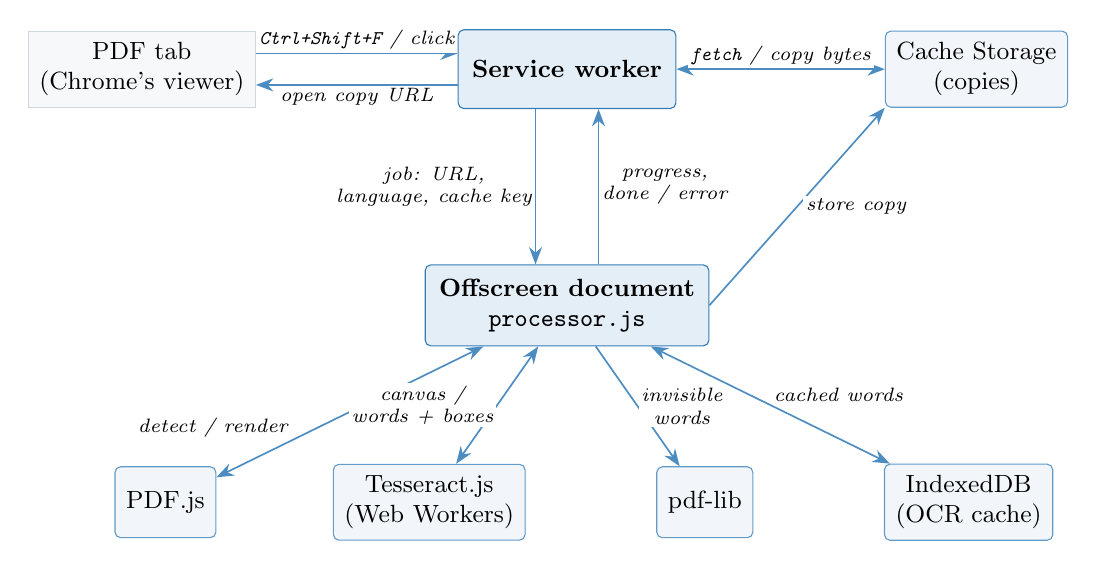
\begin{tikzpicture}[
      font=\small,
      tech/.style={rectangle, rounded corners=2pt, draw=accent!70, fill=accent!6,
                   align=center, minimum height=9mm, inner sep=4pt},
      hub/.style={rectangle, rounded corners=2pt, draw=accent!90, fill=accent!12,
                  align=center, minimum height=10mm, inner sep=5pt, font=\small\bfseries},
      io/.style={rectangle, draw=rulegray, fill=codebg, align=center,
                 minimum height=9mm, inner sep=4pt},
      a/.style={-{Stealth[length=2.2mm]}, draw=accent!80, semithick},
      b/.style={{Stealth[length=2.2mm]}-{Stealth[length=2.2mm]}, draw=accent!80, semithick},
      lbl/.style={font=\scriptsize\itshape, fill=white, inner sep=1pt, align=center},
    ]
    \node[io]   (tab)    at (-5.4, 0)   {PDF tab\\(Chrome's viewer)};
    \node[hub]  (sw)     at (0, 0)      {Service worker};
    \node[tech] (cs)     at (5.2, 0)    {Cache Storage\\(copies)};
    \node[hub]  (off)    at (0, -3.0)   {Offscreen document\\\code{processor.js}};
    \node[tech] (pdfjs)  at (-5.1, -5.5) {PDF.js};
    \node[tech] (tess)   at (-1.75, -5.5) {Tesseract.js\\(Web Workers)};
    \node[tech] (pdflib) at (1.75, -5.5) {pdf-lib};
    \node[tech] (idb)    at (5.1, -5.5) {IndexedDB\\(OCR cache)};

    \draw[a] ([yshift=2mm]tab.east) -- node[lbl,above]{\code{Ctrl+Shift+F} / click} ([yshift=2mm]sw.west);
    \draw[a] ([yshift=-2mm]sw.west) -- node[lbl,below]{open copy URL} ([yshift=-2mm]tab.east);
    \draw[b] (sw) -- node[lbl,above]{\code{fetch} / copy bytes} (cs);
    \draw[a] ([xshift=-4mm]sw.south) -- node[lbl,left]{job: URL,\\language, cache key} ([xshift=-4mm]off.north);
    \draw[a] ([xshift=4mm]off.north) -- node[lbl,right]{progress,\\done / error} ([xshift=4mm]sw.south);
    \draw[a] (off.east) -- node[lbl,right=2pt]{store copy} (cs.south west);
    \draw[b] (off) -- node[lbl,pos=0.72,above left]{detect / render} (pdfjs);
    \draw[b] (off) -- node[lbl,left]{canvas /\\words + boxes} (tess);
    \draw[a] (off) -- node[lbl,right]{invisible\\words} (pdflib);
    \draw[b] (off) -- node[lbl,above right]{cached words} (idb);
  \end{tikzpicture}
  \caption{Integration view. The service worker talks to the browser (trigger,
           tab navigation, serving the copy); the offscreen document drives the
           libraries. Arrow labels name the data crossing each boundary;
           double-headed arrows indicate request--response pairs. The finished
           copy reaches the viewer through Cache Storage, not through messages.}
  \label{fig:integration}
\end{figure}

\section{System Design and Architecture}
\label{sec:design}

\subsection{Overview}
\proj{} is structured as a \emph{pipeline} that converts an incoming PDF request
into searchable DOM text. A PDF navigation is intercepted and redirected to a
custom viewer; the viewer renders each page, checks whether it paints raster images or lacks
extractable text, recovers image text with OCR where needed, normalizes coordinates,
and injects an invisible text layer that the browser's find feature can search.
Figure~\ref{fig:pipeline} shows the end-to-end flow.

\begin{figure}[p]
  \centering
  \vspace*{6mm}
  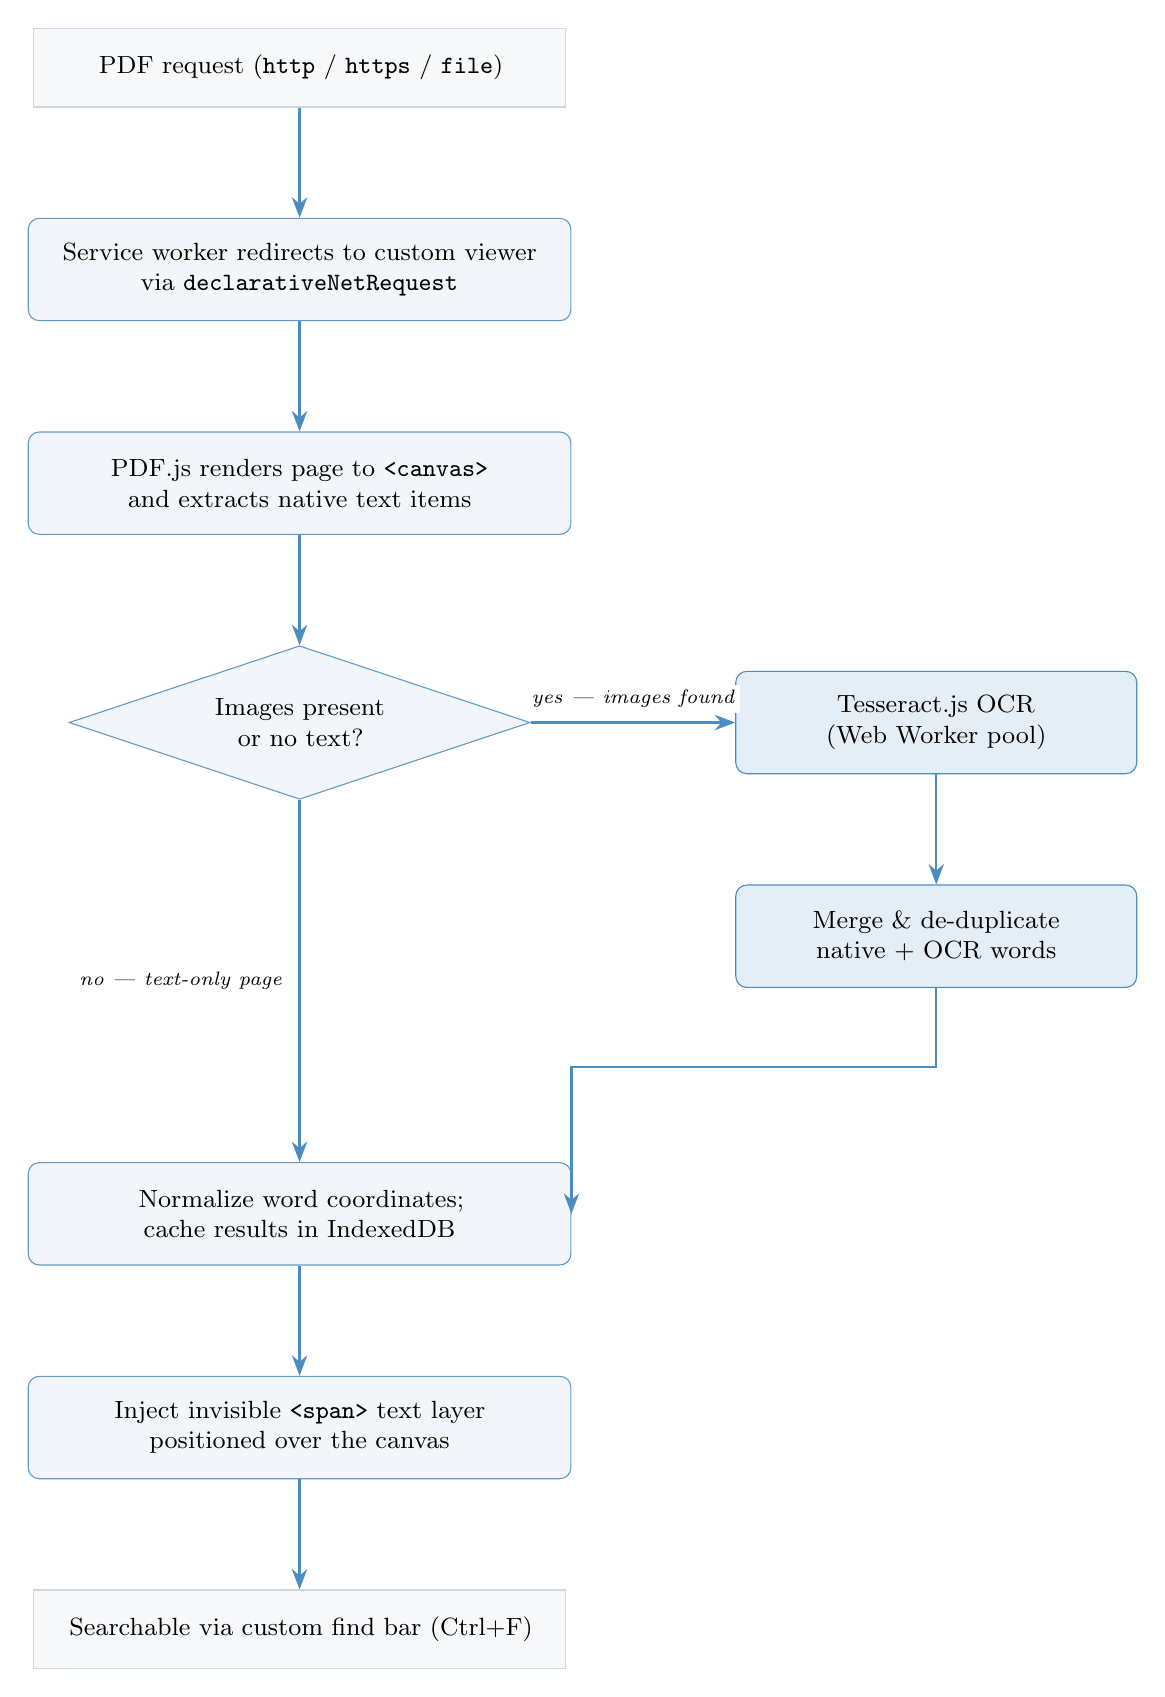
\begin{tikzpicture}[
      %% Generous vertical gap between every node
      node distance=14mm,
      %% Main-column boxes
      box/.style={rectangle, rounded corners=4pt, draw=accent!70, fill=accent!6,
                  text width=6.4cm, align=center, minimum height=13mm,
                  font=\small, inner sep=7pt},
      %% OCR-branch boxes (slightly shaded to mark the conditional path)
      side/.style={rectangle, rounded corners=4pt, draw=accent!80, fill=accent!12,
                   text width=4.6cm, align=center, minimum height=13mm,
                   font=\small, inner sep=7pt},
      dec/.style={diamond, aspect=3.0, draw=accent!70, fill=accent!6,
                  align=center, font=\small, inner sep=3pt},
      io/.style={rectangle, draw=rulegray, fill=codebg, text width=6.4cm,
                 align=center, font=\small, minimum height=10mm, inner sep=5pt},
      arr/.style={-{Stealth[length=2.6mm]}, draw=accent!80, thick},
      lbl/.style={font=\scriptsize\itshape, fill=white, inner sep=2pt},
    ]

    %% ── Left (main) column ──────────────────────────────────────────────────
    \node[io]  (req)    {PDF request
                         (\code{http} / \code{https} / \code{file})};

    \node[box, below=of req]    (sw)
      {Service worker redirects to custom viewer\\
       via \code{declarativeNetRequest}};

    \node[box, below=of sw]     (render)
      {PDF.js renders page to \code{<canvas>}\\
       and extracts native text items};

    \node[dec, below=14mm of render, text width=3.2cm] (dec)
      {Images present\\or no text?};

    \node[box, below=46mm of dec] (norm)
      {Normalize word coordinates;\\
       cache results in IndexedDB};

    \node[box, below=of norm]   (inject)
      {Inject invisible \code{<span>} text layer\\
       positioned over the canvas};

    \node[io,  below=of inject] (search)
      {Searchable via custom find bar
       ($\mathrm{Ctrl}{+}\mathrm{F}$)};

    %% ── Right (OCR) branch ──────────────────────────────────────────────────
    \node[side, right=26mm of dec] (ocr)
      {Tesseract.js OCR\\
       (Web Worker pool)};

    \node[side, below=14mm of ocr] (merge)
      {Merge \& de-duplicate\\
       native + OCR words};

    %% ── Arrows ──────────────────────────────────────────────────────────────
    \draw[arr] (req)    -- (sw);
    \draw[arr] (sw)     -- (render);
    \draw[arr] (render) -- (dec);

    %% "no" path: straight down the left column, skips OCR
    \draw[arr] (dec.south)
      -- node[lbl, left=4pt] {no --- text-only page}
      (norm.north);

    %% "yes" path: right to OCR branch
    \draw[arr] (dec.east)
      -- node[lbl, above=3pt] {yes --- images found}
      (ocr.west);

    \draw[arr] (ocr) -- (merge);

    %% merge rejoins main column via a clean L-shaped connector
    \draw[arr] (merge.south) -- ++(0,-10mm) -| (norm.east);

    \draw[arr] (norm)   -- (inject);
    \draw[arr] (inject) -- (search);
  \end{tikzpicture}
  \vspace*{4mm}
  \caption{End-to-end processing pipeline. Each page is rendered and its native text
           extracted. If the page contains raster image operators \emph{or} has no
           extractable text (right branch), Tesseract.js runs OCR on a high-resolution
           offscreen canvas and the results are merged with any native text, dropping
           duplicates. Text-only pages skip OCR and pass straight to normalization
           (left path). Both paths converge at coordinate normalization before the
           invisible text layer is injected over the canvas.}
  \label{fig:pipeline}
\end{figure}

\subsection{Components}
\begin{description}[leftmargin=1.4em, style=nextline]
  \item[Request interception] A service worker registers a dynamic
        \code{declarativeNetRequest} rule on install that matches URLs ending in
        \code{.pdf} and redirects them to \code{viewer.html}, preserving the
        original URL as a query parameter.
  \item[Custom viewer] A self-contained HTML/JS page that owns rendering, OCR
        orchestration, the text layer, and the find UI.
  \item[Rendering] PDF.js rasterizes each page to a canvas, lazily and at the
        device pixel ratio for crisp output.
  \item[Text detection] For each page the viewer asks PDF.js for its text content
        and operator list to decide whether OCR is required.
  \item[OCR] A pool of Tesseract.js Web Workers recognizes text on image pages,
        returning words with bounding boxes.
  \item[Normalization \& caching] Word coordinates are normalized to the unit
        square and cached in IndexedDB so results are reusable across zoom levels
        and sessions.
  \item[Text-layer injection] Invisible, individually-scaled \code{<span>}
        elements are positioned over the canvas.
  \item[Search] A custom find bar searches the injected text and draws highlight
        overlays.
\end{description}

\subsection{The Coordinate-Mapping Problem}
The hardest part of the system is geometric. Text originates in up to four
distinct coordinate spaces, and the injected overlay must align with the rendered
page in all of them simultaneously:

\begin{center}
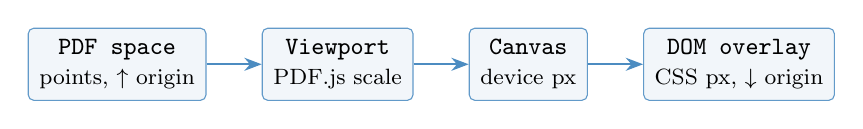
\begin{tikzpicture}[
    sp/.style={rectangle, rounded corners=2pt, draw=accent!70, fill=accent!6,
               align=center, font=\small\ttfamily, minimum height=9mm,
               inner sep=4pt},
    a/.style={-{Stealth[length=2.2mm]}, draw=accent!80, thick}]
  \node[sp] (pdf) {PDF space\\\footnotesize\rmfamily points, $\uparrow$ origin};
  \node[sp, right=7mm of pdf] (vp) {Viewport\\\footnotesize\rmfamily PDF.js scale};
  \node[sp, right=7mm of vp] (cv) {Canvas\\\footnotesize\rmfamily device px};
  \node[sp, right=7mm of cv] (dom) {DOM overlay\\\footnotesize\rmfamily CSS px, $\downarrow$ origin};
  \draw[a] (pdf) -- (vp);
  \draw[a] (vp) -- (cv);
  \draw[a] (cv) -- (dom);
\end{tikzpicture}
\end{center}

PDF space uses typographic points with a bottom-left origin; the PDF.js viewport
applies a scale (and any page rotation); the canvas backing store is further
scaled by the device pixel ratio for high-DPI sharpness; and the DOM overlay uses
CSS pixels with a top-left origin. A glyph recovered or extracted in one space
must be drawn at the corresponding location in the overlay, or search highlights
and text selection drift away from the visible characters.

For \emph{native} PDF text, PDF.js supplies, per item, an affine transform
$M_{\text{item}}$ and the viewport's transform $M_{\text{vp}}$ (which already
folds in page rotation). The glyph's full matrix in device space is their product
\begin{equation}
  M \;=\; M_{\text{vp}}\, M_{\text{item}},
  \qquad
  M=\begin{bmatrix} a & c & e\\ b & d & f \\ 0 & 0 & 1\end{bmatrix},
  \label{eq:matmul}
\end{equation}
from which the baseline angle and device-space font height follow directly:
\begin{equation}
  \theta = \operatorname{atan2}(b,\,a),
  \qquad
  h = \sqrt{c^{2}+d^{2}} .
  \label{eq:angle}
\end{equation}
Because rotation falls out of the matrix in Eq.~\eqref{eq:angle}, rotated pages
and rotated text are handled without special cases. The span's top-left corner is
obtained by stepping from the baseline origin $(e,f)$ up by the ascent
$h_a \approx 0.8\,h$ along the text direction.

For \emph{OCR} text, Tesseract reports pixel bounding boxes in the
high-resolution OCR canvas. These are normalized to the unit square by dividing
by the OCR canvas dimensions,
\begin{equation}
  \tilde{x} = \frac{x}{W_{\text{ocr}}},\qquad
  \tilde{y} = \frac{y}{H_{\text{ocr}}},
  \label{eq:normalize}
\end{equation}
so the cached result is independent of the resolution at which OCR happened. At
draw time they are denormalized into the text layer's CSS-pixel space using the
\emph{viewport} dimensions---not the DPR-scaled canvas dimensions---so the
invisible text and the visible page share one coordinate system.

\subsection{Key Design Decisions}
Four decisions shape the rest of the system and are justified where they appear
in Section~\ref{sec:impl}:

\begin{enumerate}
  \item \textbf{Never modify the original PDF.} The system is a strictly
        read-only render plus an overlay: the source file's bytes and format are
        left untouched, and all recovered text lives in a separate, invisible DOM
        layer. This constraint, fixed from the outset, rules out any
        rewrite-the-PDF approach and is the reason searchability is added
        \emph{around} the document rather than \emph{into} it.
  \item \textbf{Inject real text instead of intercepting search.} This reuses the
        browser's indexing, matching, and (optionally) highlighting, and keeps
        recovered text selectable and copyable.
  \item \textbf{Separate the OCR image from the display image.} Display fidelity
        and OCR legibility have different requirements, so the page is rendered
        twice: once for the screen at the device pixel ratio, and once offscreen
        at high resolution purely for recognition.
  \item \textbf{Lazy rendering with background indexing.} Pages render as they
        approach the viewport for responsiveness, while a separate idle-time pass
        guarantees that off-screen pages still become searchable.
\end{enumerate}

\section{Development Process: Phased Implementation}
\label{sec:process}

\proj{} was built incrementally, one phase at a time, with each phase shipped and
tested before the next began. Two principles held from the start: the original
PDF is \textbf{never modified}, and the headline capability, \textbf{finding text
inside images}, had to be as close to ``100\% findable'' as possible. A third
arrived late and reshaped the whole system: the user must see \textbf{nothing but
Chrome's own viewer}. This section records how the work was planned, how it
actually unfolded, and the reasoning at each step.

\subsection{Planning: The Initial Estimate}
Before writing code, the work was broken into seven phases with rough effort
estimates (Table~\ref{tab:planned}). Two were flagged up front as the likely
time-sinks: the \emph{invisible text-layer overlay} (the coordinate-alignment
problem) and \emph{intercepting Chrome's built-in PDF viewer}, which is sandboxed
and cannot simply be scripted.

\begin{table}[ht]
  \centering
  \caption{Initial seven-phase plan drawn up before implementation began. Phases~5
           and~6 were flagged as the expected time-sinks; Phase~6 was ultimately
           pulled forward and solved first.}
  \label{tab:planned}
  \renewcommand{\arraystretch}{1.2}
  \begin{tabularx}{\textwidth}{@{}clX@{}}
    \toprule
    \textbf{\#} & \textbf{Planned phase} & \textbf{Note} \\
    \midrule
    1 & Extension scaffolding (MV3) & Manifest, service worker, content-script wiring \\
    2 & PDF.js rendering pipeline & Pages to canvas; worker setup in an extension context \\
    3 & Tesseract.js OCR & Plumbing OCR into the async page pipeline \\
    4 & Per-page text detection & \code{getTextContent()} check --- quick \\
    5 & Invisible text-layer overlay & \emph{Hardest:} PDF$\leftrightarrow$canvas$\leftrightarrow$DOM coordinate alignment \\
    6 & Intercept Chrome's PDF viewer & \emph{Hidden complexity:} sandboxed viewer; must redirect \\
    7 & Polish, edge cases, testing & --- \\
    \bottomrule
  \end{tabularx}
\end{table}

\subsection{Execution: How the Build Actually Unfolded}
Execution diverged from the plan in two instructive ways. First, viewer
interception (planned as Phase~6) turned out to be a \emph{prerequisite} for
everything else---you cannot render or overlay anything until you control the
page---so it was solved first, folded into Phase~1. Second, ``OCR accuracy''
was not a single step but the dominant theme of the back half of the project: it
expanded into several phases as the README roadmap and real test feedback
exposed new failure modes. The phases below are the build as it actually
happened.

\medskip
\noindent\textbf{Foundation.}
\begin{description}[leftmargin=1.4em, style=nextline, itemsep=4pt]
  \item[Phase 1 --- Extension skeleton \& PDF interception.] Built the MV3
        manifest, service worker, content script, and an empty viewer, then made
        the service worker redirect \code{.pdf} navigations to that viewer.
        \emph{Why first:} Chrome opens PDFs in its own sandboxed viewer that
        scripts cannot reach, so gaining control of the page is the true
        starting point---and it establishes the read-only-overlay architecture.
        \emph{Revealed:} a viewer that shows nothing yet $\rightarrow$ Phase~2.
  \item[Phase 2 --- PDF.js rendering pipeline.] Bundled PDF.js locally (to satisfy
        the MV3 CSP) and rendered each page to a canvas, switching to a
        \emph{dynamic} redirect rule so the original URL survives as
        \code{?url=}. \emph{Friction:} \code{file://} security origins and the
        \code{getDocument} URL parameter both needed care. \emph{Revealed:} pages
        display but nothing is searchable $\rightarrow$ Phase~3.
  \item[Phase 3 --- Text detection, OCR \& the invisible overlay.] The heart of
        the project: detect native text with \code{getTextContent()}, OCR image
        pages with Tesseract.js in a worker, and inject invisible spans over the
        canvas. \emph{Key pivot:} the first design was \emph{either/or} (use
        native text, else OCR), but a page containing the same word both as native
        text \emph{and} inside an image matched only the native copy---image text
        was lost. The design changed to \emph{both}: always inject native text,
        then OCR images and merge only the non-duplicate words (text-aware
        de-duplication). \emph{Revealed:} OCR re-ran on every load $\rightarrow$
        Phase~4.
  \item[Phase 4 --- IndexedDB caching.] Cache each page's words once, keyed per
        document, with coordinates normalized to $[0,1]$ so the cache survives
        any zoom level. \emph{Why:} OCR is the expensive step, so it should be a
        one-time cost. \emph{Revealed:} language data still implied a CDN
        $\rightarrow$ Phase~5.
  \item[Phase 5 --- Fully offline.] Bundled the LSTM language model and pointed
        Tesseract's \code{langPath} at it, removing the last network dependency.
        \emph{Why:} privacy, reliability, and offline use---no document data ever
        leaves the machine.
\end{description}

\noindent\textbf{Refinement} (working through the README roadmap and test feedback).
\begin{description}[leftmargin=1.4em, style=nextline, itemsep=4pt]
  \item[Phase 6 --- OCR accuracy: correction variants.] Added confidence
        filtering, edge-noise trimming, and digit$\rightarrow$letter correction
        variants (\code{he11o}$\rightarrow$\code{hello}) injected as search-only
        spans. \emph{Thought:} native find is exact-match, so rather than
        fuzzy-matching at query time, widen the \emph{stored} text.
  \item[Phase 7 --- Rotated pages.] Derived each glyph's angle and size from the
        \code{viewport.transform}\,$\times$\,\code{item.transform} matrix and
        rotated the spans to match, so rotation is handled by the math rather
        than special cases (Section~\ref{sec:design}).
  \item[Phase 8 --- Multi-language OCR.] Added an English/Danish selector with a
        per-language cache, so switching languages reprocesses independently and
        non-destructively.
  \item[Phase 9 --- Performance on large PDFs.] Introduced lazy,
        viewport-driven rendering, idle-time background indexing, and
        \emph{parallel} OCR via a worker scheduler. \emph{Thought:} a single
        serial OCR worker was the real bottleneck; the roadmap's ``GPU
        acceleration'' proved not actionable (Tesseract.js has no GPU path and
        already uses the SIMD WASM core), so parallelism was the available win.
  \item[Phase 10 --- Readability \& search UX.] Driven directly by user testing:
        the text layer was made selectable/copyable; a measure-and-scale fix
        aligned each invisible span to its exact width after selection and search
        landed on the wrong characters (``\,Where is\,''$\rightarrow$``\,Where is
        the b\,''); and the native find bar---which flashed the invisible layer
        as oversized doubled text---was replaced by a custom find bar with
        translucent highlights, $\uparrow/\downarrow$ navigation, and a distinct
        active-match style for colourful pages.
  \item[Phase 11 --- OCR image preprocessing.] The final push on the
        ``100\% findable'' goal, targeting the cases still failing: sparse-text
        segmentation recovered \emph{tables}; a high-resolution (3000\,px) OCR
        canvas recovered \emph{small} text; and a percentile contrast stretch
        plus unsharp mask attacked \emph{low-contrast and blurred} text (the
        cache format version was bumped to invalidate stale results).
        \emph{Thought:} decouple the OCR image from the display image and push
        recognition as far as preprocessing allows---while accepting a hard
        ceiling on genuinely low-resolution source images.
\end{description}

\medskip
\noindent\textbf{Production} (preparing for release).
\begin{description}[leftmargin=1.4em, style=nextline, itemsep=4pt]
  \item[Phase 12 --- Activation model: from automatic to on demand.] The biggest
        late change reversed Phase~1's founding decision. Until now the extension
        intercepted \emph{every} PDF navigation with \code{declarativeNetRequest}
        and forced it into the custom viewer. Dogfooding on ordinary text PDFs
        exposed the flaw: Chrome's native PDF viewer is a sandboxed plugin, so
        replacing it threw away its entire toolbar and right-click menu
        (thumbnails, rotate, print, download, Google~Lens, $\dots$)---none of which
        a DOM viewer can reproduce---while for an already-searchable text PDF the
        extension added nothing. \emph{Decision:} keep Chrome's native viewer as
        the default and invoke the OCR viewer \emph{on demand} via a keyboard
        shortcut (\code{Ctrl+Shift+F}) or the toolbar icon, toggling back on a
        second press. \emph{Why:} the extension's value is real only for image and
        scanned PDFs, and those are precisely the documents where the native
        toolbar matters least---so scoping activation to them preserves the native
        experience everywhere else (decision~\ref{dec:ondemand}). \emph{Side
        benefit:} dropping interception also removed the \code{declarativeNetRequest}
        and \code{storage} permissions and the catch-all content script, leaving a
        much smaller, easier-to-review permission footprint.
  \item[Phase 13 --- Imitating the native viewer.] Even on demand, the OCR viewer
        was still a \emph{different} viewer, so the next effort made it look and
        behave like Chrome's: a Chrome-style toolbar with zoom and page
        navigation, a find bar restyled after Chrome's (match counter,
        $\uparrow/\downarrow$, Esc/Enter/Shift+Enter), Chrome's yellow and orange
        highlights, the find bar opening already focused, and a return to the
        native viewer at the same page via \code{\#page=N}. A new search engine
        matched phrases across OCR word boundaries (the old one matched only
        inside a single span), and background indexing stopped freezing in hidden
        tabs once rendering used PDF.js's \code{print} intent, which is not paced
        by \code{requestAnimationFrame}. \emph{Revealed:} the user's verdict was
        that an imitation is not the original---they wanted ``same behaviour as
        that of original \dots\ and same design and view also'', with no
        different view and no change to the PDF's format $\rightarrow$ Phase~14.
  \item[Phase 14 --- Native viewer only: the searchable-scan sandwich.] The
        custom viewer was deleted outright (about 1{,}300 lines). In its place, an
        offscreen document OCRs the PDF and uses pdf-lib to write the recognized
        words into a \emph{copy} as invisible text (\code{3~Tr}), each word sized
        and squeezed so Chrome's highlight covers it (Section~\ref{sec:coords});
        the tab then switches to that copy in Chrome's own viewer. Progress moved
        to a badge on the toolbar icon and the OCR language to the icon's
        right-click menu. \emph{Thought:} the only way to give the user Chrome's
        exact interface is to give Chrome a file it can search itself. This also
        reinterpreted ``never modify the PDF'': the original is still never
        touched, and the copy's visible content was verified identical by pixel
        comparison (0 of 2{,}298{,}825 pixels differed). \emph{Gap:} the pipeline
        was tested in a browser tab, but the final tab switch was not verified in
        Chrome itself.
  \item[Phase 15 --- First use in the user's browser.] Loading the build into the
        user's own Chrome surfaced two problems. OCR crashed inside the offscreen
        document in Tesseract's \emph{relaxed-SIMD} WebAssembly core: Tesseract.js
        chooses that core when a \code{WebAssembly.validate()} probe accepts it,
        but on this Chrome and Apple Silicon combination the probe passed and
        execution trapped. The vendored worker was patched so the probe always
        reports relaxed SIMD as unavailable, falling back to the mature SIMD core.
        Separately, \code{chrome://extensions/shortcuts} showed the Mac shortcut
        (\code{Cmd+Shift+F}) as ``Not set''; that was only explained in
        Phase~16.
  \item[Phase 16 --- Release hardening, verified in real Chrome.] A review before
        publishing to the Chrome Web Store added, for the first time, an
        automated end-to-end test that loads the \emph{packaged} extension into a
        throwaway Chrome profile and drives it through the DevTools
        protocol~\cite{cdp}. It found that the core feature had never worked:
        Chrome silently refuses to navigate a website tab to an extension's
        \code{blob:} URL, so the tab never switched to the searchable copy. Copies
        are now served from the extension's own origin by the service worker
        (decision~\ref{dec:serve}). The same review and tests found and fixed:
        \begin{itemize}[nosep]
          \item OCR collapsing into noise on sparse pages: the contrast stretch's
                dark point fell inside the background, amplifying JPEG noise up
                to $127\times$; the stretch gain is now capped
                (Section~\ref{sec:impl}).
          \item A release zip that omitted the \code{offscreen/} folder, because
                the packaging script still listed the deleted viewer.
          \item The Mac shortcut: Chrome leaves the suggested \code{Cmd+Shift+F}
                unassigned (\code{chrome.commands.getAll()} reports no shortcut),
                so the default is now Control+Shift+F, making the shortcut
                \code{Ctrl+Shift+F} on every platform.
          \item PDFs whose URL lacks ``.pdf'' were ignored; the extension now
                accepts any web or file URL and checks the file's \code{\%PDF-}
                signature.
          \item Danish letters were stripped from word edges (``på'' was stored
                as ``p''), because word trimming only recognized \code{a-z}; it
                now uses Unicode letter classes.
          \item OCR results keyed by URL could be applied to a changed file; the
                cache now keys by a SHA-256 of the content and prunes itself
                (decision~\ref{dec:hash}).
          \item Silent failures: encrypted PDFs, non-PDF pages, and disabled file
                access now show a red badge with an explanation; the success
                badge is set only after the copy loads, because Chrome clears a
                tab's badge when it navigates.
          \item Unbounded resources: pdf.js documents are destroyed after each
                job and idle OCR workers are released
                (decision~\ref{dec:bounded}); unused Tesseract builds were
                removed, shrinking the package from 22.5\,MB to 8.5\,MB.
          \item Store requirements: a manifest description within 132 characters,
                a privacy policy, and listing material.
        \end{itemize}
        \emph{Thought:} unit-level checks had proved the pipeline; only driving
        the real browser proved the product.
\end{description}

\subsection{Plan versus Reality}
The original instinct that the \emph{overlay} would be the hardest part was
correct---coordinate alignment, the native-versus-image de-duplication, and the
measure-and-scale fitting absorbed the most iteration. The estimate was wrong in
its \emph{shape}, though: ``OCR'' looked like one tidy phase but became the
project's centre of gravity, because the headline promise (find \emph{any} text
in \emph{any} image) is exactly the kind of goal that surfaces a long tail of
real-world failure modes---rotation, tables, multiple languages, blur, low
contrast, small type. Each was its own phase, and each was reached by shipping
the previous one and watching where it still fell short.

The plan was also wrong about where the project would end. It assumed a custom
viewer throughout; in the end the custom viewer, its overlay, and its find bar
were all deleted, and the coordinate work moved from the DOM into the PDF itself.
The hardest late problems were not algorithms but \emph{platform behaviour}: what
Chrome lets an extension do with its sandboxed viewer, with blob URLs, with
keyboard shortcuts, and with toolbar badges. None of these showed up in tests of
the pipeline alone; each surfaced only when the real browser was in the loop.

\section{Implementation}
\label{sec:impl}

This section walks through the pipeline stage by stage. Code excerpts are drawn
from the extension's source and lightly trimmed for space.

\subsection{Extension Structure and Activation}
The extension is a Manifest~V3 package with no content scripts. Its content
security policy permits \code{wasm-unsafe-eval} so the bundled Tesseract
WebAssembly core can run, and the OCR engine, language data, PDF.js and pdf-lib
are all bundled---no CDN fetch occurs at runtime.

Activation is on demand (decision~\ref{dec:ondemand}). Two entry points---the
toolbar icon (\code{action.onClicked}) and a keyboard shortcut
(\code{commands.onCommand}, \code{Ctrl+Shift+F} on every platform)---run one
handler (Listing~\ref{lst:activate}). On a searchable copy it restores the
original, whose URL is carried in the copy's \code{src} parameter. Otherwise it
starts the offscreen document and sends it the job, including the copy URL and
cache key the service worker has chosen, so that the naming of copies lives in
one place.

\begin{lstlisting}[caption={On-demand activation: one handler for the toolbar icon and the shortcut. It restores the original when the tab shows a copy, and otherwise starts a job (\code{service-worker.js}).}, label={lst:activate}]
async function toggle(tab) {
  // Showing a searchable copy? Restore the original PDF.
  if (isCopyUrl(tab.url)) {
    const original = originalOf(tab.url);
    await dropSwap(tab.id);
    await deleteCopy(tab.url);
    if (original) chrome.tabs.update(tab.id, { url: original });
    return;
  }
  if (!isFetchableUrl(tab.url)) return badgeError(tab.id, "open a PDF in this tab first");

  badge(tab.id, "...", "Making this PDF searchable...");
  await ensureOffscreen();
  const url = tab.url.split("#")[0];
  const copyUrl = newCopyUrl(url);   // chrome-extension://<id>/searchable/<uuid>/<name>?src=<url>
  chrome.runtime.sendMessage({ type: "fii-process", tabId: tab.id, url,
    lang: await getLang(), copyUrl, cache: COPY_CACHE, cacheKey: copyKey(copyUrl) });
}
chrome.action.onClicked.addListener((tab) => toggle(tab));
chrome.commands.onCommand.addListener((cmd, tab) => { if (cmd === "toggle-search") toggle(tab); });
\end{lstlisting}

Local \code{file://} PDFs additionally require the per-extension ``Allow access to
file URLs'' setting; if it is off, the handler shows a red badge explaining this
and opens the extension's details page, where the toggle lives.

\subsection{Download, Validation, and Identity}
The offscreen document downloads the PDF again from the tab's URL with
\code{credentials: "include"}, so that PDFs on sites the user is signed in to
return the same file the tab shows. The trigger accepts \emph{any} web or file
URL, because many PDFs are served from addresses without ``.pdf'' (for example
\code{arxiv.org/pdf/2111.03017} or \code{download.php?id=7}). Validation therefore
happens on the bytes: a PDF must contain the signature \code{\%PDF-} within its
first kilobyte. A page that returns HTML is reported as ``not a PDF (or a
sign-in page)''.

The bytes are then loaded twice, by PDF.js (for analysis and rendering) and by
pdf-lib (for writing), while \code{crypto.subtle.digest} computes their SHA-256 in
parallel. If either library reports encryption, the job ends with a clear
message: pdf-lib cannot write into encrypted files. pdf-lib's
\code{EncryptedPDFError} is transpiled ES5, so \code{instanceof} does not
recognize it and the check matches its message instead. The PDF.js loading task
is destroyed in a \code{finally} block, because the offscreen document lives all
session and would otherwise keep every processed document in memory.

\subsection{Text Detection}
For each page the processor first calls \code{getTextContent()}. OCR runs when
the page paints raster images \emph{or} when no text is extractable at all (a page
may be a scan, or have its text converted to vector outlines---both invisible to
\code{getTextContent()}). Image detection inspects the operator list:

\begin{lstlisting}[caption={Image detection: scans the PDF.js operator list for raster paint opcodes to decide whether a page needs OCR (\code{processor.js}).}, label={lst:hasimages}]
const IMAGE_OPS = new Set([
  pdfjsLib.OPS.paintImageXObject,      pdfjsLib.OPS.paintInlineImageXObject,
  pdfjsLib.OPS.paintImageMaskXObject,  pdfjsLib.OPS.paintImageXObjectRepeat,
]);
async function pageHasImages(page) {
  const opList = await page.getOperatorList();
  return opList.fnArray.some((fn) => IMAGE_OPS.has(fn));
}
\end{lstlisting}

If image detection fails it \emph{fails open}---assuming images are present---on
the principle that an unnecessary OCR pass is cheaper than silently missing text.

\subsection{OCR Rendering and Preprocessing}
Pages that need OCR are rendered to an offscreen canvas about 3000\,px wide
($\approx$360\,DPI for a Letter page), with PDF.js's \code{print} intent so that
rendering is not paced by \code{requestAnimationFrame}, which never fires in a
hidden document. The canvas is released immediately after recognition.

Before recognition, the image is converted to grayscale and preprocessed to
attack the two hardest cases, low contrast and blur:
\begin{enumerate}
  \item \textbf{Gain-capped contrast stretch.} With $P_{2}$ and $P_{98}$ the 2nd
        and 98th percentiles of the luminance histogram, every gray level $v$ is
        remapped as
        \begin{equation}
          v' = 255 - 255\,\frac{P_{98} - v}{R},
          \qquad
          R = \max\bigl(R_{\min},\; P_{98} - P_{2}\bigr),
          \quad R_{\min} = 96 .
          \label{eq:stretch}
        \end{equation}
        When the percentiles are far apart this is the classic stretch
        ($P_2\mapsto 0$, $P_{98}\mapsto 255$). The floor $R_{\min}$ matters on
        mostly blank pages: when text covers less than 2\% of the pixels, $P_2$
        is itself background. On the first test pages $P_2$ was 233--238 against
        $P_{98}=240$, so the uncapped stretch multiplied contrast by up to
        $127\times$, turned faint JPEG noise into black speckle, and made one page
        unreadable. Anchoring at $P_{98}$ keeps the background white, and the
        floor limits the gain to $255/96 \approx 2.7$.
  \item \textbf{Unsharp mask.} Edges are re-sharpened as
        $\text{sharp} = g + \alpha\,(g - g_{\text{blur}})$ with $\alpha=1$, where
        $g_{\text{blur}}$ comes from a separable box blur implemented with a
        sliding-window sum, so its cost is $O(n)$ independent of radius.
\end{enumerate}
Tesseract performs its own binarization afterward, so this stage only needs to
hand it a clean, high-contrast grayscale image.

\subsection{OCR Engine Orchestration}
Recognition runs through a Tesseract.js \emph{scheduler} that distributes pages
across a pool of Web Workers. The worker count scales with CPU cores but is
capped, because each worker loads its own copy of the language model:
\begin{equation}
  N_{\text{workers}} = \max\!\big(1,\ \min(4,\ \texttt{hardwareConcurrency}-1)\big).
\end{equation}
The processor keeps $N_{\text{workers}}$ pages in flight at once. JavaScript is
single-threaded, so pdf-lib edits to different pages interleave safely; only the
rendering and recognition awaits overlap. Workers use \emph{sparse text} page
segmentation, which finds table cells, captions, and scattered text far better
than the default layout analysis. Three language modes are supported---\code{eng},
\code{dan}, and \code{eng+dan}---with one worker pool per language. Sixty seconds
after the job queue empties, all pools are terminated to free their memory; they
are recreated on the next job.

\subsection{Post-Processing for Findability}
Because native find performs exact substring matching, fuzzy matching is
impossible at search time; the post-processing stage improves the \emph{stored}
text instead. It drops near-zero-confidence noise, trims non-letter junk from
word edges (with Unicode letter classes, so Danish words keep their
\textit{æ}, \textit{ø} and \textit{å}), and emits a \emph{correction variant}
for words that look like digit/letter confusions (\code{he11o}\,$\to$\,\code{hello},
\code{ca5h}\,$\to$\,\code{cash}). Tokens that are more than half digits are left
alone as genuine numbers or codes:

\begin{lstlisting}[caption={Emitting a correction variant for OCR tokens with likely digit/letter confusions (\code{ocr-postprocess.js}).}, label={lst:variant}]
const DIGIT_TO_LETTER = { "0":"o","1":"l","5":"s","6":"b","8":"b","9":"g","2":"z" };
out.push({ text, bbox: w.bbox });                 // the word as recognized
const variant = correctionVariant(text);          // null unless mostly letters + some digits
if (variant && variant !== text)
  out.push({ text: variant, bbox: w.bbox, variant: true });
\end{lstlisting}

The earlier DOM viewer injected both forms and hid the variant from selection.
Inside a real PDF there is no such distinction: two words at one spot would
double Chrome's match count and duplicate copied text. The processor therefore
embeds a single form, preferring the corrected variant, since it is what the
image most likely says.

\subsection{Writing the Invisible Layer}
Each recognized word is mapped into PDF user space as described in
Section~\ref{sec:coords} and de-duplicated against the page's existing text.
The survivors are appended to the page's content stream as one invisible text
object each (Listing~\ref{lst:embed}). The whole block is wrapped in
\code{q}/\code{Q} so its text state cannot leak into anything drawn later.
Helvetica's WinAnsi encoding covers English and Danish; a word containing a
character it cannot encode is skipped rather than failing the page.

\begin{lstlisting}[caption={Writing one invisible, width-matched text object per word with pdf-lib (\code{embed.js}).}, label={lst:embed}]
for (const wd of words) {
  const encoded = font.encodeText(wd.text);
  const natural = font.widthOfTextAtSize(wd.text, wd.h);
  const squeeze = Math.max(1, Math.min(1000, (wd.w / natural) * 100));  // Tz, percent
  const cos = Math.cos(wd.angle), sin = Math.sin(wd.angle);
  ops.push(
    PDFLib.beginText(),
    PDFLib.setTextRenderingMode(PDFLib.TextRenderingMode.Invisible),     // 3 Tr
    PDFLib.setFontAndSize(fontKey, wd.h),
    PDFLib.setCharacterSqueeze(squeeze),
    PDFLib.setTextMatrix(cos, sin, -sin, cos, wd.x, wd.y),
    PDFLib.showText(encoded),
    PDFLib.endText(),
  );
}
page.pushOperators(PDFLib.pushGraphicsState(), ...ops, PDFLib.popGraphicsState());
\end{lstlisting}

The document is then saved with its metadata untouched, and the bytes are
stored in Cache Storage as an \code{application/pdf} response under the key the
service worker supplied.

\subsection{Caching}
Recognized words are normalized to the unit square (Eq.~\eqref{eq:normalize}) and
stored in IndexedDB under \code{<sha256>::<lang>::<page>}. Because the key is the
file's content hash, the same PDF reached through two different URLs is
recognized once, and a different file at a familiar URL is never matched to
stale words. Empty results are cached too, so text-only pages are not re-examined.
Each record carries a \emph{format version}, bumped whenever the OCR pipeline
changes, and a last-used timestamp. A cache hit refreshes the timestamp, and
after every job the oldest records are deleted until at most 2{,}000 pages
remain.

\subsection{Serving and Cleaning Up the Copy}
When the job is done, the service worker checks that the tab still shows the
same PDF (the user may have moved on), records which copy the tab shows, and
navigates it to the copy URL. Chrome requests that URL from the extension, and
the service worker's \code{fetch} handler answers it (Listing~\ref{lst:serve}).
Chrome sees an \code{application/pdf} response and opens its own viewer; because
the path ends in the original file name, the tab title is unchanged. The success
badge is set only after the tab finishes loading, because Chrome clears a tab's
badge whenever it navigates.

\begin{lstlisting}[caption={Serving searchable copies at the extension's own URLs. Cache Storage only accepts http(s) keys, so copies are stored under a placeholder origin with the same path (\code{service-worker.js}).}, label={lst:serve}]
self.addEventListener("fetch", (event) => {
  const url = new URL(event.request.url);
  if (url.origin !== self.location.origin || !url.pathname.startsWith("/searchable/")) return;
  event.respondWith(serveCopy(url));
});
async function serveCopy(url) {
  const hit = await (await caches.open(COPY_CACHE)).match(COPY_KEY_ORIGIN + url.pathname);
  if (hit) return hit;
  // The copy is gone (e.g. the browser restarted): fall back to the original PDF.
  const src = url.searchParams.get("src");
  if (src && isFetchableUrl(src)) return Response.redirect(src, 302);
  return new Response("This searchable copy is no longer available.", { status: 404 });
}
\end{lstlisting}

Copies are deleted when the user restores the original, when their tab
navigates elsewhere or closes, and when the browser starts. A tab that returns to
a deleted copy---through session restore or the browser's history---simply
redirects to the original PDF.

\section{Results and Evaluation}
\label{sec:results}

This evaluation is qualitative and behavioral: it characterizes what the system
achieves and how its architecture behaves, rather than reporting formal accuracy
or timing benchmarks, which are identified as future work in
Section~\ref{sec:limitations}.

\subsection{Functional Outcomes}
The system meets its central goal: scanned and image-based PDFs that return
nothing to in-page search become fully searchable in the browser. Specifically:
\begin{itemize}
  \item \textbf{Scanned PDFs become searchable.} Pages with no text layer are
        OCR'd and their text injected, so queries match content that was
        previously invisible to search.
  \item \textbf{Mixed pages are handled.} Pages combining native text with text
        baked into images expose both, with duplicates removed so a word is never
        double-counted.
  \item \textbf{Rotated text aligns.} Because rotation is recovered from the
        transform matrix (Eq.~\eqref{eq:angle}) rather than special-cased,
        highlights and selection track rotated pages and rotated runs.
  \item \textbf{Selection and copy work.} Injected text is real DOM text, so
        users can not only find but also select and copy recovered content;
        search-only correction variants are excluded from copy to avoid
        duplication.
  \item \textbf{Fully offline.} OCR engine, language models, and PDF.js are
        bundled, so no document data leaves the machine and the extension works
        without a network connection.
\end{itemize}

\subsection{Architectural Behavior}
The performance-oriented design choices produce the following observable
behavior:

\begin{table}[ht]
  \centering
  \caption{Design mechanisms and the behavior they produce.}
  \label{tab:results}
  \renewcommand{\arraystretch}{1.3}
  \begin{tabularx}{\textwidth}{@{}lX@{}}
    \toprule
    \textbf{Mechanism} & \textbf{Observed effect} \\
    \midrule
    Lazy, viewport-driven rendering & Large documents open immediately;
      only near-viewport pages do work up front. \\
    Idle-time background indexing & Off-screen pages still become searchable,
      scheduled during idle time so scrolling is never blocked. \\
    Web Worker OCR pool & Recognition runs off the main thread on several pages
      at once; the interface stays responsive during OCR. \\
    High-resolution OCR canvas + preprocessing & Small text inside images is
      legible to the recognizer independent of on-screen zoom. \\
    IndexedDB caching (normalized coords) & A document is OCR'd once; re-opening
      or re-zooming it is instant and correct at any scale. \\
    Correction variants & Common digit/letter misreads remain findable by their
      true spelling. \\
    \bottomrule
  \end{tabularx}
\end{table}

\subsection{Component Complexity}
Table~\ref{tab:scope} summarizes the relative implementation complexity of each
component. The coordinate-mapping and DOM-overlay subsystems dominate: they are
where most of the subtle, correctness-critical logic lives.

\begin{table}[ht]
  \centering
  \caption{Relative complexity by component.}
  \label{tab:scope}
  \renewcommand{\arraystretch}{1.25}
  \begin{tabular}{@{}lc@{}}
    \toprule
    \textbf{Component} & \textbf{Complexity} \\
    \midrule
    PDF rendering (PDF.js)            & Medium \\
    OCR pipeline (Tesseract.js)       & Medium \\
    Chrome extension integration      & Medium \\
    Coordinate mapping                & High \\
    DOM text-overlay system           & High \\
    \bottomrule
  \end{tabular}
\end{table}

\subsection{Discussion}
The results validate the project's central thesis: by converting documents into
real, well-positioned DOM text, the system inherits the browser's mature search
behavior almost for free, and the engineering effort concentrates where the real
difficulty lies---geometric alignment and keeping a CPU-heavy workload off the
critical path. The accuracy layer (high-resolution rendering, preprocessing, and
correction variants) measurably widens what is findable in practice, though it
cannot fully overcome poor source scans; this is examined next.

\section{Limitations and Future Work}
\label{sec:limitations}

\subsection{Limitations}
\begin{description}[leftmargin=1.4em, style=nextline]
  \item[OCR is not perfect.] Recognition errors propagate into search. Because
        native find is exact, a misread character can make a word unfindable by
        its true spelling. Correction variants mitigate the most common
        digit/letter confusions but do not cover the general case.
  \item[Cost scales with the document.] Recognition is CPU-bound and runs on the
        client. Very large or very dense documents take correspondingly longer to
        fully index, even though lazy rendering keeps the document immediately
        readable and caching makes subsequent loads instant.
  \item[Complex layouts can misalign.] Multi-column text, unusual fonts, and
        heavy graphical backgrounds can produce slight overlay drift or
        degraded recognition.
  \item[Device-dependent performance.] Throughput depends on the number of CPU
        cores and the device's overall capability, since the worker pool scales
        with available concurrency.
  \item[Scope is currently PDF-centric.] Image text on ordinary web pages is not
        yet handled; the content script that would address this is presently a
        placeholder.
\end{description}

\subsection{Future Work}
\begin{itemize}
  \item \textbf{Higher OCR accuracy.} Richer post-processing---dictionary-based
        correction, confidence-weighted variants, and language-model
        re-ranking---to reduce unfindable misreads beyond the current
        digit/letter mapping.
  \item \textbf{Better rotation and skew handling.} Automatic deskew before
        recognition for photographed or imperfectly-scanned pages.
  \item \textbf{Broader language support.} Additional bundled language models and
        automatic script detection.
  \item \textbf{Acceleration.} Exploiting GPU/WebAssembly SIMD acceleration and
        preprocessing whole documents in the background to shorten time-to-fully-
        searchable on large files.
  \item \textbf{General web-page image text.} Extending the pipeline, via the
        content script, to make text inside ordinary \code{<img>} elements
        searchable, not just PDFs.
  \item \textbf{Quantitative evaluation.} A benchmark suite measuring recognition
        accuracy (e.g.\ character/word error rate) and per-page latency across a
        corpus of representative scanned documents, to turn the qualitative
        results of Section~\ref{sec:results} into reproducible numbers.
\end{itemize}

\section{Conclusion}
\label{sec:conclusion}

\proj{} demonstrates that the most effective way to make a scanned document
searchable in the browser is not to build a search engine, but to \emph{make the
document into real text} and let the browser do what it already does well. In its
final form, the extension adds no interface at all. On demand, it recognizes the
text in a PDF's images on the user's own machine, writes it into a copy of the
file as an invisible layer, and lets Chrome's own viewer and Chrome's own find
bar do the rest. The original file is never modified, and the copy looks exactly
like it.

Reaching that form took two reversals. The project began with a custom viewer
that overlaid invisible DOM text on PDF.js renderings, which required a careful
coordinate pipeline, measure-and-scale fitting, and a custom find bar. The first
reversal made the viewer opt-in, because replacing Chrome's PDF experience for
every document cost more than it gave. The second removed the viewer entirely,
because any imitation of Chrome's interface was still not Chrome's interface. The
geometric work did not disappear; it moved into the PDF, where each word is placed
in user space at the right size, angle and width for Chrome's own highlight to
cover it.

The last phase supplied the project's most practical lesson. Every component
had been tested, yet the product did not work: Chrome would not open the copy
from where it was stored. The bug became visible only when the packaged extension
was driven through the real browser. That test now protects the release, and its
fixes---serving copies from the extension's origin, content-addressed caching, a
contrast stretch that cannot amplify noise, and bounded resources---are what make
the extension ready for others to use.

More broadly, the project illustrates a reusable principle for client-side
engineering: bridge a new capability (OCR) into an existing, battle-tested
substrate (the PDF format and the browser's viewer) rather than re-implementing
that substrate---and verify the result where users will actually meet it.


% ---------- References --------------------------------------------------------
\clearpage
\addcontentsline{toc}{section}{References}
\bibliographystyle{ieeetr}
\bibliography{references}

\end{document}
